\begin{frame}{command}
    \begin{figure}
    	\centering
    	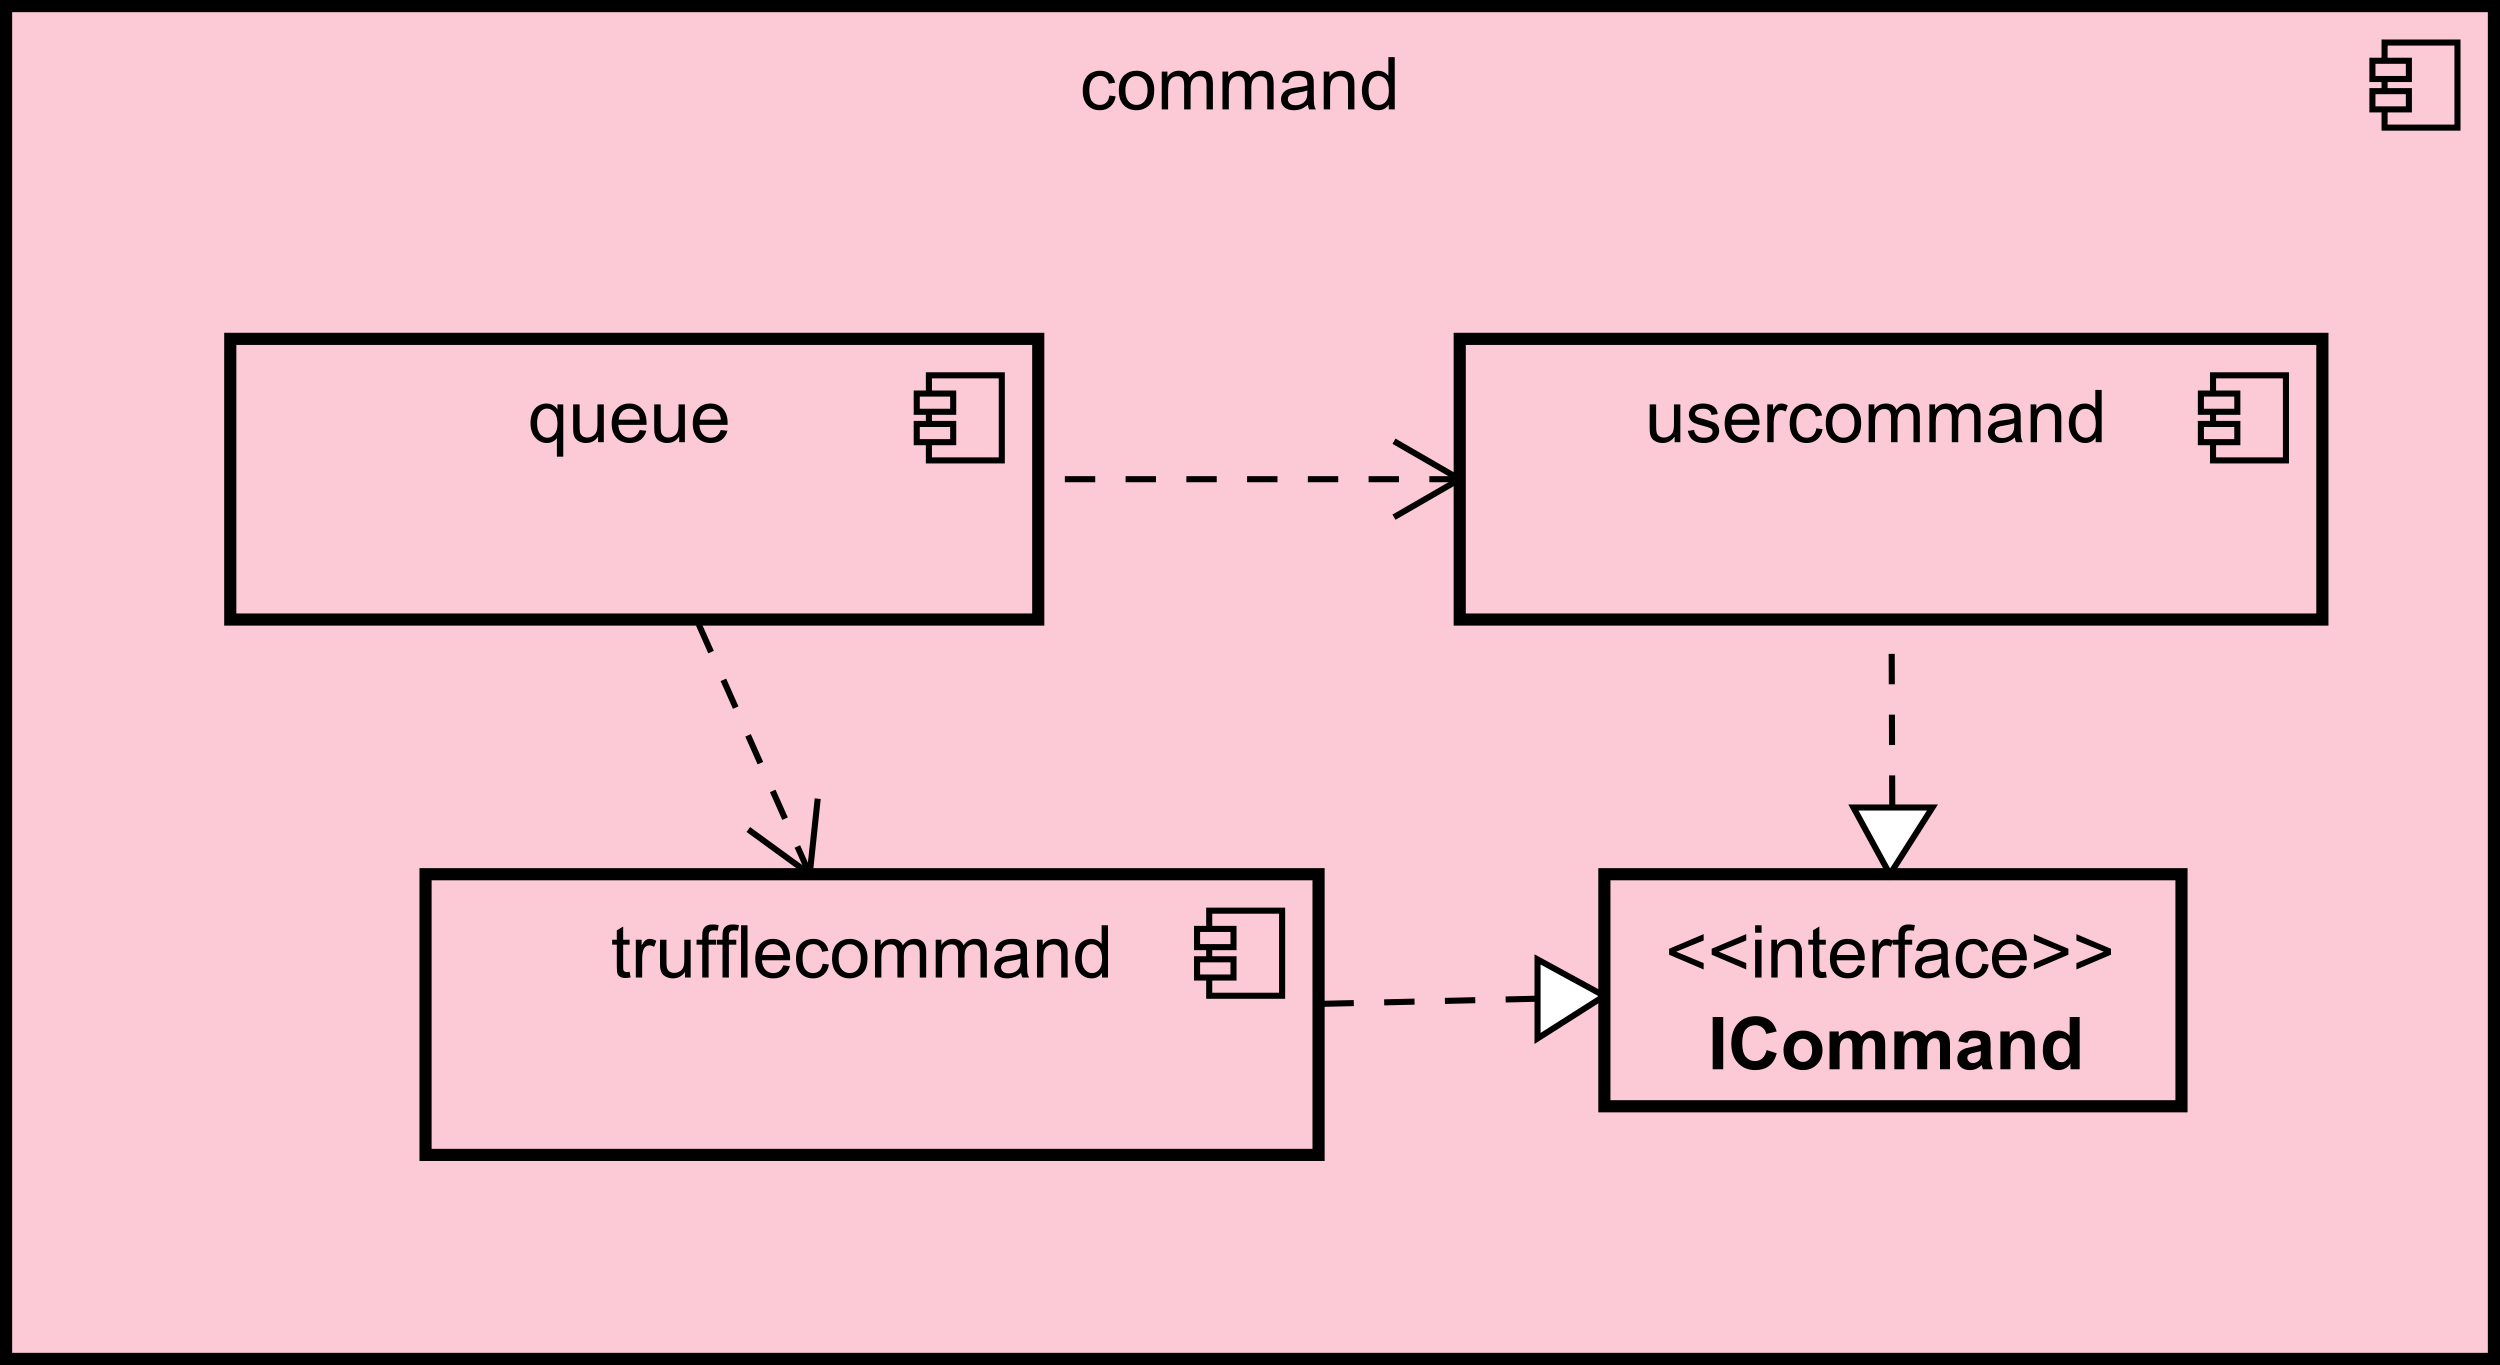
\includegraphics[width=\textwidth]{./images/command.png}
    \end{figure}
\end{frame}

\begin{frame}{command}
    \begin{itemize}[<+->]
      \item Aufgaben
        \begin{itemize}
          \item Kommunikation im Programm
          \item Beinhalten die auszuführenden Aufgaben
        \end{itemize}
      \item Entwurfsentscheidung
        \begin{itemize}
          \item Kurze Lebensdauer
          \item Gute Anwendung für das Observer Pattern
          \item Verbergen von Implementierung
          \item Erweiterbare Funktionalität
        \end{itemize}
    \end{itemize}
\end{frame}